\documentclass[journal,13pt,twocolumn]{IEEEtran}

\usepackage{setspace}
\usepackage{gensymb}
\counterwithin{equation}{section}
\singlespacing

\newcommand{\myvec}[1]{\ensuremath{\begin{pmatrix}#1\end{pmatrix}}}
\newcommand{\mydet}[1]{\ensuremath{\begin{vmatrix}#1\end{vmatrix}}}

\usepackage[cmex10]{amsmath}
\usepackage{amsthm}
\usepackage{mathrsfs}
\usepackage{txfonts}
\usepackage{stfloats}
\usepackage{bm}
\usepackage{cite}
\usepackage{cases}
\usepackage{subfig}
\usepackage{longtable}
\usepackage{multirow}
\usepackage{mathtools}
\usepackage{steinmetz}
\usepackage{tikz}
\usepackage{circuitikz}
\usepackage{verbatim}
\usepackage{tfrupee}
\usepackage[breaklinks=true]{hyperref}
\usepackage{tkz-euclide} % loads  TikZ and tkz-base
%\usetkzobj{all}
\usetikzlibrary{calc,math}
\usepackage{listings}
    \usepackage{color}                                            %%
    \usepackage{array}                                            %%
    \usepackage{longtable}                                        %%
    \usepackage{calc}                                             %%
    \usepackage{multirow}                                         %%
    \usepackage{hhline}                                           %%
    \usepackage{ifthen}                                           %%
  %optionally (for landscape tables embedded in another document): %%
    \usepackage{lscape}     
\usepackage{multicol}
\usepackage{chngcntr}
\usepackage{pgfplots}
\usepackage{pgfplotstable}
\pgfplotsset{compat=1.7}
\usepackage{tikz}
\DeclareMathOperator*{\Res}{Res}
\renewcommand\thesection{\arabic{section}}
\renewcommand\thesubsection{\thesection.\arabic{subsection}}
\renewcommand\thesubsubsection{\thesubsection.\arabic{subsubsection}}

\renewcommand\thesectiondis{\arabic{section}}
\renewcommand\thesubsectiondis{\thesectiondis.\arabic{subsection}}
\renewcommand\thesubsubsectiondis{\thesubsectiondis.\arabic{subsubsection}}

\DeclarePairedDelimiter\abs{\lvert}{\rvert} % \abs{} for numerisk værdi
\DeclarePairedDelimiter\norm{\lVert}{\rVert}
\makeatletter
\let\oldabs\abs
\def\abs{\@ifstar{\oldabs}{\oldabs*}}
\let\oldnorm\norm
\def\norm{\@ifstar{\oldnorm}{\oldnorm*}}
\makeatother
\renewcommand{\vec}[1]{\mathbf{#1}}
\newcommand{\bignorm}[1]{\Bigl \| #1 \Bigr \| #1}
\hyphenation{op-tical net-works semi-conduc-tor}
\def\inputGnumericTable{}                                 %%

\lstset{
frame=single, 
breaklines=true,
columns=fullflexible
}
\begin{document}
\title{Assignment 4} 
\author{Shweta Verma} 
\maketitle
\newpage
\bigskip
\begin{abstract}
This document determines the value of $k$ for which the given equation represents two straight lines.
\end{abstract}
\section{\textbf{Problem}}
For what value of $k$ does the equation 
\begin{align}
\vec{x}^T \myvec{6 && k/2 \\ k/2 && -3} \vec{x} + \myvec{4 && 5}\vec{x} -2 = 0
\end{align}
represent a pair of straight lines?
\section{\textbf{Solution}}
The given equation can be represented as:
\begin{align}
\vec{x}^T \myvec{a && h \\ h && b} \vec{x} + \myvec{2g && 2f}\vec{x} +c = 0
\end{align}
Comparing equation (1.1) and equation (2.1) we get\\
a=6, b=-3, h=k/2, g=2, f=5/2, c=-2\\
Discriminant of the equation (2.1)
\begin{align}
\Delta = \mydet{a && h && g\\ h && b && f\\ g && f && c}
\end{align}
Substituting the values in equation (2.2)
\begin{align}
\Delta = \mydet{6 && k/2 && 2\\ k/2 && -3 && 5/2\\2 && 5/2 && -2}
\end{align}
If the equation (1.1) represents a pair of straight lines\\
then Discriminant is zero
\begin{align}
\Delta = 0
\end{align}
\begin{align}
\implies \mydet{6 && k/2 && 2\\ k/2 && -3 && 5/2\\2 && 5/2 && -2} = 0
\end{align}
\begin{align}
k^2 + 10k + 21 = 0
\end{align}
\begin{align}
k = -3,-7
\end{align}

\begin{figure}
   \centering
   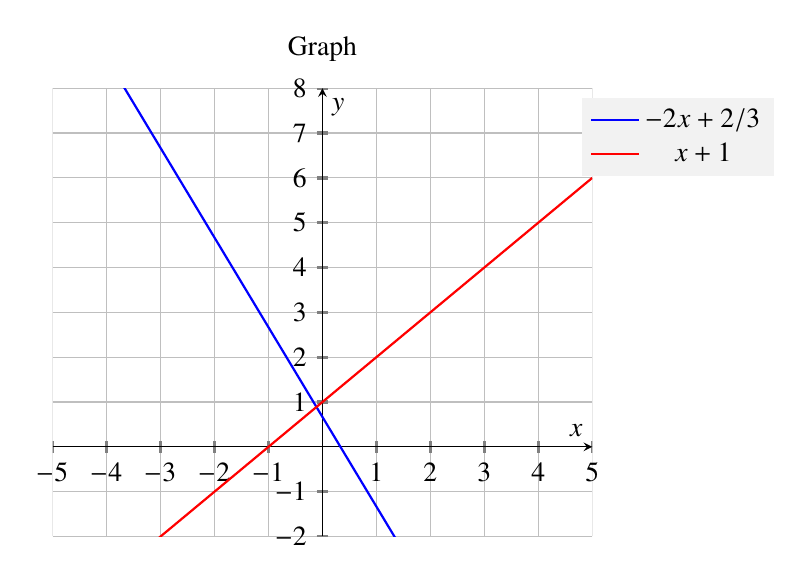
\begin{tikzpicture}
   \begin{axis}[
   legend style={anchor=north west,draw=none,fill=gray!10},
   axis lines=middle,
   grid=major,
   xmin=-5,
   xmax=5,
   ymin=-2,
   ymax=8,
   title=Graph,
   xlabel={$x$},
   ylabel={$y$},
   xtick={-5,-4,...,5},
   ytick={-2,-1,...,8},
   tick style={very thick}
   ]
   \addplot[blue,thick]{-2*x+2/3};
   \addlegendentry{$-2x+2/3$}
   \addplot[red,thick]{x+1};
   \addlegendentry{$x+1$}
   \end{axis}
   \end{tikzpicture}
   \caption{This is a plot of pair of straight lines in (1.1)}
   \end{figure}
\end{document} 